\section{Kernspins und Quantenzahlen}
\textbf{Warum sind die Kernspins der beiden Rubidiumisotope unterschiedlich? Welche Quantenzahlen existieren im Grundzustand und den ersten beiden angeregten Zuständen für die beiden Rubidiumisotope und welche F-Quantenzahlen resultieren daraus?}\\

Der Kernspins des $^{85}$Rb beträgt $I_{85}=5/2$.
Der Kernspins des $^{87}$Rb beträgt $I_{87}=3/2$.
Diese unterscheiden sich da man Isotope von Rubidium hat.
Das $^{87}$Rb-Atom hat 2 Neutronen mehr.
Der Kernspin $I$ ist die Summe der Summe von Spin und Bahndrehimpuls aller Nukleonen.\\

Für die verschiedenen Quantenzahlen folgt:
\begin{figure}[h]
    \centering{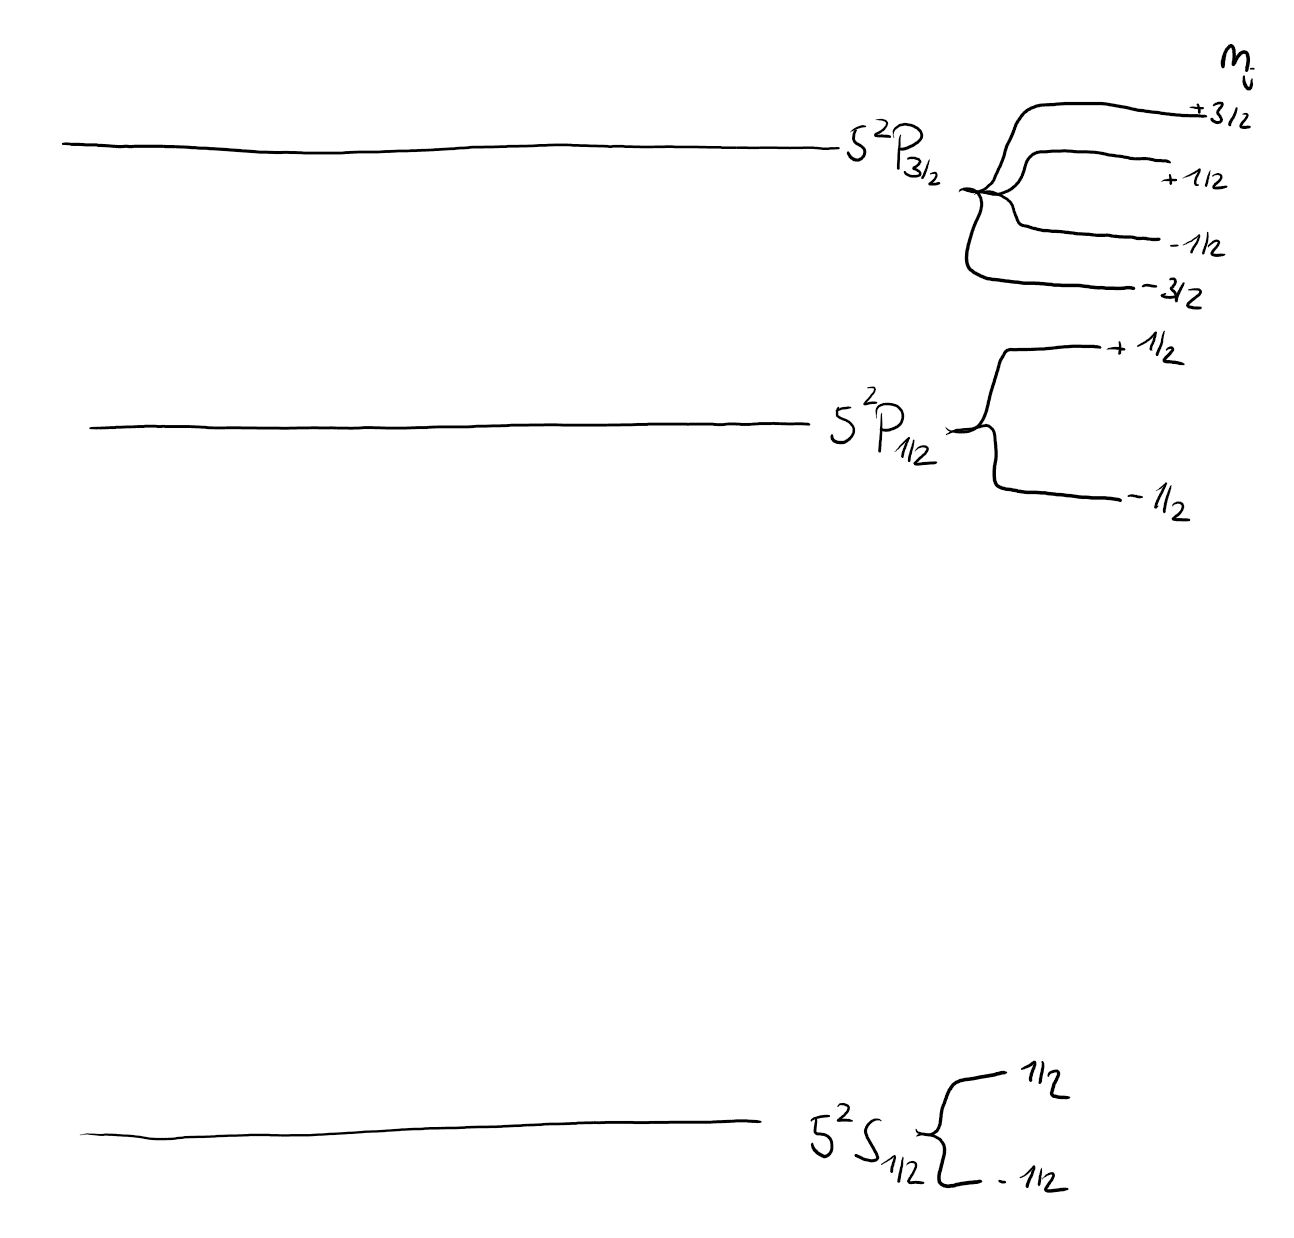
\includegraphics[width=0.4\textwidth]{FzV/87.png}}
    \caption{Quantenzahlen von Rubidium}
\end{figure}

Die F-Quantenzahlen kann man wie folgt bestimmen:
\begin{equation}
    F=\left|J-I\right|,\left|J-I\right|+1,..,J+I-1,J+I
\end{equation}
Somit hat $^{85}$Rb eine F Quantenzahl von 2 bis 3 und $^{87}$Rb eine F Quantenzahl von 1 bis 2 für den $S/P_{\frac{1}{2}}$.
Für den Zustand $P_{\frac{3}{2}}$ hat $^{85}$Rb eine F Quantenzahl von 1 bis 4 und $^{87}$Rb eine F Quantenzahl von 0 bis 3.
\section{Begriffe}
\textbf{Informieren Sie sich zu den Begriffen 'natürliche Linienbreite', 'Doppel-Verbreiterung', 'homogene/inhomogen Verbreiterung' und 'Sättigungsverbreiterung'.}\\

\textbf{Natürliche Linienbreite und homogene/inhomogene Verbreiterung}\\
Die \textbf{natürliche Linienbreite} basiert auf der Energie-Zeit-Unschärferelation.
Die Bestimmung der Lebensdauer und der exakten Energie eines 
angeregten Zustandes ist nicht möglich. 
Dies führt zu einer statischen Verbreiterung der Linienbreite.\\
Unter Verbreiterungsmechanismen versteht man die Vergrößerung der Linienbreite
über die natürliche Linienbreite hinaus. Hierbei unterscheidet man zwischen zwei Arten:\\
Die \textbf{homogene Verbreiterung} tritt auf, wenn die Emissionswahrscheinlickeit für eine bestimmte Frequenz 
für alle Teilchen gleich groß ist. Hierzu zählen z.B. Druckverbreiterung und Sättigungsverbreiterung.\\
Die \textbf{inhomogen Verbreitung} tritt auf, wenn die Emissionswahrscheinlickeit für eine bestimmte Frequenz 
nicht für alle Teilchen gleich groß ist. Hierzu zählen z.B. Doppelverbreiterung.\\

\textbf{Doppelverbreiterung}\\
Dort hängt die Wahrscheinlichtkeit von der Geschwindigkeit der Moleküle ab.
Diese bewegen sich auf dem Detektor zu und wieder weg, was eine Änderung der Frequenz zur Folge hat (Doppler-Effekt).
Da nun die Geschwindigkeiten nicht gleichmäßig verteilt sind (Stefan-Boltzmann-Verteilung), kommt es zu einer inhomogenen Linienverbreiterung.\\

\textbf{Sättigungsverbreiterung}\\
Eine weitere Linienverbreiterung ist die Sättigungsverbreiterung.
Hier wächst die Linienbreite an, da der Übergangszustand durch eine Pumpe größtenteils gesättigt sind.
Tritt dies ein, werden mehr Photonen am Rand der Linie absorpiert, was zu einer homogenen Verbreiterung der Spektrallinie führt.
\section{Cross-Over Resonanzen}
\textbf{Was sind 'Cross-Over Resonanzen' und wie entstehen diese?}\\

Liegen in einem Spektrum zwei Niveaus nahe nebeneinander, so gibt es eine Überkreuzung (\textit{Cross-Over}).
Dadurch entsteht eine Weitere Linie im Spektrum.\\

Erklärt werden kann dies dadurch, dass die entgegengesetzte Dopplerverschiebung des Pump- und Abfangstrahls gleich groß, aber entgegengesetzt ist.
Dadurch tritt die Entvölkerung durch die Pumpe und Absorption durch den Abfangstrahl in den gleichen Geschwindigkeitsklassen auf, wodurch die Absorption verringert ist \citep[vgl.][]{Wiki-Dopp}.